\documentclass[10 pt,usenames,dvipsnames, oneside]{article}
\usepackage{../../../modelo-ensino-medio}



\begin{document}

\begin{center}
  \begin{minipage}[l]{3cm}
\includegraphics[width=2cm]{logo}    
\end{minipage}\hfill
\begin{minipage}[r]{.8\textwidth}
 {\Large \scshape Atividade: Pêndulo de um relógio}  
\end{minipage}
\end{center}
\vspace{.2cm}

\ifdefined\prof
%Habilidades da BNCC
% \begin{objetivos}
% \item 
% \end{objetivos}

%Caixa do Para o Professor
\begin{goals}
%Objetivos específicos
\begin{enumerate}
\item Reconhecer de fenômenos periódicos
\item Construir gráficos de fenômenos que podem ser modelados
por função periódica
\end{enumerate}

\tcblower

%Orientações e sugestões
Nesta atividade, espera-se que o aluno consiga perceber o
movimento de “sobe e desce”{} que o gráfico da função que
modela o movimento possui. Além disso, espera-se que ele
perceba que esse movimento se replica à direita quando a
variável do domínio (tempo) aumenta, sendo então diferente
dos gráficos das funções estudadas até aqui. Não há problema
de, nesse momento, o gráfico apresentar imperfeições como
por exemplo, ser construído através de segmentos de reta que
sobem e descem. A atividade seguinte, que tem um cunho
experimental possibilitará ao aluno perceber que o gráfico,
além de ter os comportamentos acima destacados, precisa ter
um formato “arredondado”, se aproximando então da curva
senóide a ser definida nas seções posteriores
\end{goals}

\bigskip
\begin{center}
{\large \scshape Atividade}
\end{center}
\fi

\textit{(Adaptado de Costa (2017))}
\label{trig-ativ1}

Alguns relógios rústicos têm um pêndulo, composto por uma bolinha presa à parte de baixo de uma haste que oscila continuamente de um lado para o outro. O fato de o pêndulo estar em movimento mostra que o relógio está em pleno funcionamento.

\begin{figure}[H]
\centering

\includegraphics[width=.25\linewidth]{trigonometricas1}
\end{figure}

Vamos estudar o comportamento da projeção do centro dessa bola numa reta horizontal localizada abaixo desse relógio, supondo que a origem dessa reta coincida com a projeção do centro da bola quando a haste do pêndulo está na posição vertical. Em outras palavras, vamos estudar as variações dos pontos da reta alcançados pela projeção do centro da bola. As imagens a seguir ilustram algumas possíveis posições do pêndulo. O centro do pêndulo está representado pelo ponto $E$; os pontos $C$ e $B$ são os pontos extremos do caminho percorrido pelo pêndulo. O ponto $O$ é aquele em que o pêndulo se encontra preso ao relógio. O ponto $F$ indica possíveis posições do pêndulo, e o ponto $G$ indica a projeção de $E$ na reta orientada a seguir. Observe as diferentes posições de $F$ ilustradas e os valores da distância entre $A$ e $G$ ($A$ é a projeção de $O$ na reta orientada). A construção no GeoGebra do movimento de um pêndulo similar a esse pode ser acessada no link \url{https://www.geogebra.org/classic/uxcqamaz}


\begin{figure}[H]
\centering

\includegraphics[width=\linewidth]{trigonometricas2}
\end{figure}

Suponha que no tempo $t$, a função que descreve o deslocamento dessa projeção seja $d(t)$. Note que, como estabelecemos uma posição como origem, esta função é considerada com sinal assumindo um valor positivo quando o pêndulo estiver à direita do segmento $OA(d(t_1)\geq0)e$ assumindo um valor negativo quando estiver à esquerda de $OA(d(t_2)\leq0)$, conforme é possível ver na ilustração acima: a distância entre $A$ e $G$ é um módulo, é absoluta; no entanto, quando consideramos a posição na reta orientada, atribuímos um sinal a essa distância.

\begin{figure}[H]
\centering

\includegraphics[width=.25\linewidth]{trigonometricas3}
\end{figure}

\ifdefined\prof
\clearpage
\else\fi
\begin{enumerate}
\item Na malha quadriculada abaixo, considere $D_{\max}$ e $E_{\max}$ o maior e o menor valor assumidos pela função $d$. Repare que $D_{\max}$ corresponde à projeção do ponto $B$ na reta horizontal, que é o ponto mais à direita que é atingido pelo centro da bolinha ao longo da oscilação do pêndulo. Da mesma forma, $E_{\max}$ corresponde à projeção de $C$, que é o ponto mais à esquerda que é atingido pelo centro da bolinha durante o movimento. Tente esboçar o gráfico da função $d(t)$, supondo que $d(0) = D_{\max}$.

\begin{figure}[H]
\centering

\resizebox{.75\linewidth}{!}
{
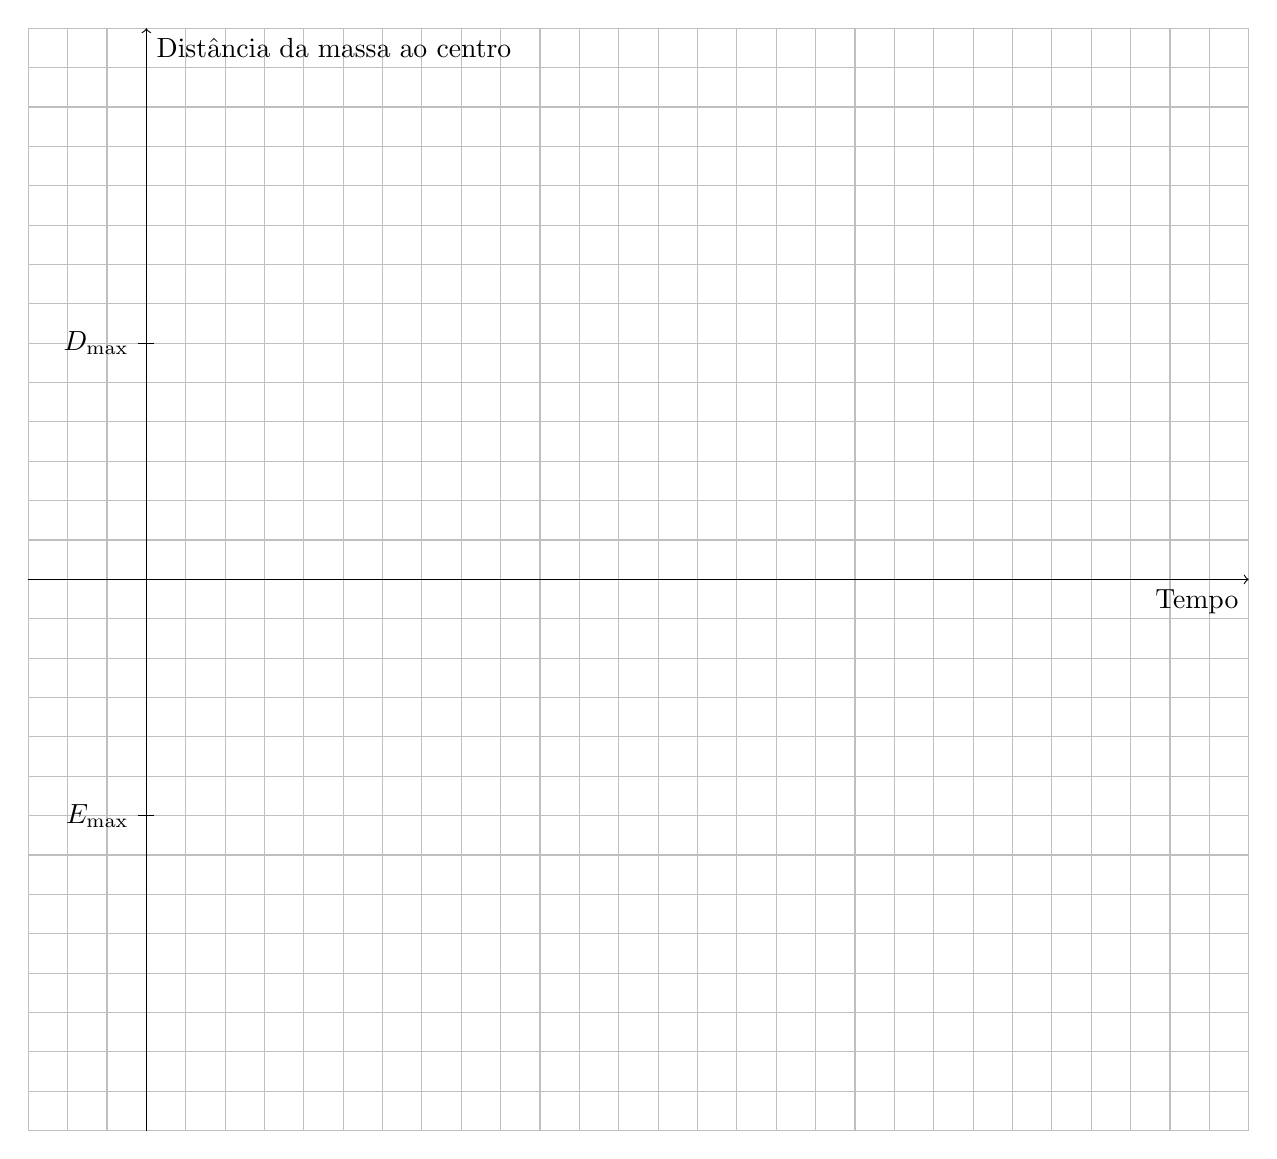
\begin{tikzpicture}
\draw [step=.5,gray!50] (-1.5,-7) grid (14,7);
\draw [->] (-1.5,0) -- (14,0) node [below left, thick] {Tempo};
\draw [->] (0,-7) -- (0,7) node [below right, thick] {Distância da massa ao centro};
\draw (.1,3) -- (-.1,3) node [left, overlay] {$D_{\max}$};
\draw (.1,-3) -- (-.1,-3) node [left, overlay] {$E_{\max}$};
\end{tikzpicture}
}
\end{figure}

\item Que aspectos você percebe que esse gráfico possui? Cite algumas diferenças entre ele e os gráficos das funções que você estudou até aqui.
\end{enumerate}

% \ifdefined\prof
% \begin{solucao}



% \end{solucao}
% \fi

\end{document}